\subsection{Fontskalierung auf Webseiten}\phantomsection\label{anhang:webFontScaling}
Beispielsweise produziert die folgende~\hyperref[fig:anhang:webFontScaling]{HTML-Notation} bei einer Skalierung im Browser von 120 Prozent (Abbildung~\ref{fig:anhang:webFontScaling:bild1}) und 50 Prozent (Abbildung~\ref{fig:anhang:webFontScaling:bild2}) jeweilig zwei verschiedene PDF (unter welchen nur Zweitere alle textlichen Inhalte offenbart). Ähnliches kann auch innerhalb \TeX{} geschehen, sollte 

\begin{figure}[h!]
\begin{Verbatim}[breaklines=true]
<html>
    <head>
        <title>Example</title>
        <style>
            /*formatting options are: none and black*/
            .t{
                font-size:13em;
                height:50%;
            }
            /*formatting option: none = no background, black, courier*/
            .t#none{
                font-family: 'Courier New', Courier, monospace;
            }
            /*formatting option: black = black background, white, serif*/
            .t#black{
                background-color:black;
                color:white;
                margin-top: -2em;
            }
        </style>
    </head>
    <body>
        <div class="t" id="none">Test</div>
        <div class="t" id="black">Test2</div>
    </body>
</html>
\end{Verbatim}
\caption{HTML-Beschreibung einer Webseite mit zwei Textflächen}
\label{fig:anhang:webFontScaling}
\end{figure}

\newpage

\begin{figure}[h!t]
    \centering
    \caption{Um die Dokumente von der restlichen Papierfläche abzugrenzen wurden schwarze Rahmen mittels Ti\textit{k}Z hinzugefügt.}
    \begin{subfigure}[t]{.4\textwidth}% Skaliert Höhe der PDF automatisch mit auf 40%; jedoch nicht \textheight
        \centering
        \begin{tikzpicture}
            \draw (0,0) rectangle (.4\textwidth,.564\textwidth);% Wir haben unserer Unterfigur nur die Info gegeben, dass die (Unter-) Figur 40 % Breite aufder Textfläche bekommt, nicht wie hoch die Figur ist. \textheight könnte demnach noch die gesamte Höhe sein. Wir wollen uns jedoch auf eine PDF beschränken, welche DINa4 folgt.
            % Habe grob gerundet. Wollte mich mal kurz wie ein Ingenieur fühlen
            % Nicht Pixel-perfect, jedoch Logik stimmt und man könnte den exakten Wert zu Not in \TeX berechnen (siehe package: https://ctan.math.illinois.edu/macros/latex/contrib/calculator/calculator.pdf)
            
\includegraphics[width=.4\textwidth]{appendices/fontscalingexample1.pdf};
        \end{tikzpicture}
        \caption{~\hyperref[fig:anhang:webFontScaling]{Zuvorige HTML-Beschreibung} liefert bei einer Browser-Skalierung von 120$\%$ obige Graphik}\label{fig:anhang:webFontScaling:bild1}
    \end{subfigure}
    ~~~
    \begin{subfigure}[t]{.4\textwidth}
        \centering
        \begin{tikzpicture}
        \draw (0,0) rectangle (.4\textwidth,.564\textwidth);
        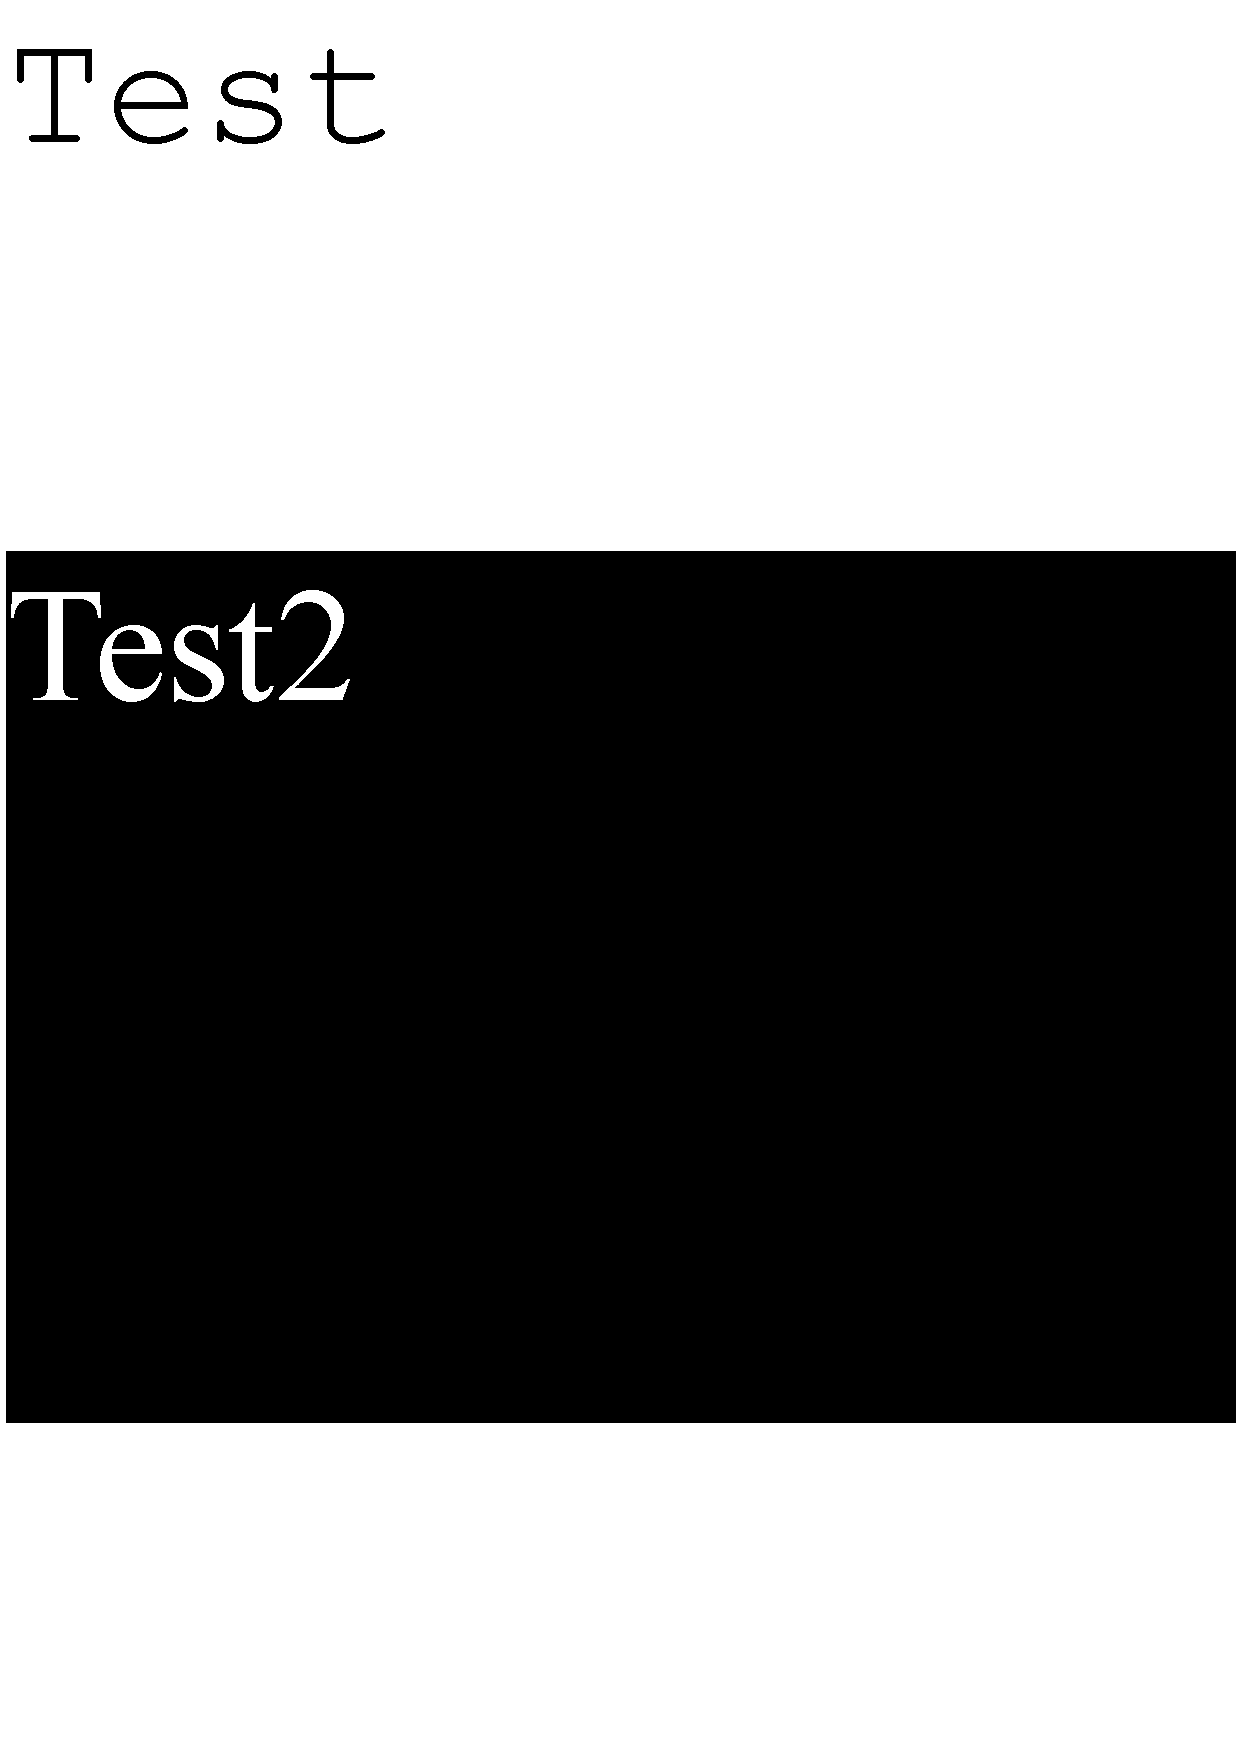
\includegraphics[width=.4\textwidth]{appendices/fontscalingexample2.pdf}
        \end{tikzpicture}
        \caption{~\hyperref[fig:anhang:webFontScaling]{Zuvorige HTML-Beschreibung} liefert bei einer Browser-Skalierung von 50$\%$ obige Graphik}\label{fig:anhang:webFontScaling:bild2}
    \end{subfigure}
\end{figure}